\documentclass{article}
\usepackage[utf8]{inputenc}
\usepackage[T1]{fontenc}
\usepackage{graphicx}
\usepackage{algorithm}
\usepackage{algpseudocode}

\usepackage{listings}
\usepackage{xcolor}
\usepackage[margin=2.5cm]{geometry}
\usepackage{float}

\usepackage{amssymb} %Ajoute des symboles mathématiques comme R, Z, forall, exists, etc....

\lstdefinestyle{monstyle}{
    backgroundcolor=\color{white},
    commentstyle=\color{gray},
    keywordstyle=\color{blue},
    numberstyle=\tiny\color{gray},
    basicstyle=\ttfamily\small,
    breaklines=true,
    numbers=left,
    numbersep=5pt,
    frame=single,
}
\lstset{style=monstyle}

\title{Rapport TD n°1 : Programmation impérative}
\author{Derrez Lorenzo}

\begin{document}
\maketitle

\section*{\textbf{Exercice 0}}

\begin{lstlisting}[language=C, caption ={Print Hello World}]
    #include <stdio.h>
    int main(int argc, char* argv[]){
        printf("Hello world\n"); 
        return 0; 
    }
    // Output : Hello world
\end{lstlisting}

\section*{\textbf{Exercice 1}}

\begin{lstlisting}[language=C, caption={PGCD}]
    // Q1 : 
int pgcd_rec(int a, int b){
    if (b == 0){
        return a; 
    }
    else{
        int r = a%b; 
        return pgcd_rec(b, r); 
    }
     
}

//Q3 :
int pgcd_iter(int a, int b){
    ///
}

// Test : 
int main(int argc, char* argv[]){
    int x1 = 15; 
    int x2 = 3; 
    int t1 = pgcd_rec(x1, x2); 
    printf("Test 1 result : %d\n", t1); 
    
    int y1 = 4; 
    int y2 = 8; 
    int t2 = pgcd_rec(y1, y2); 
    printf("Test 2 result : %d\n", t2);

    int z1 = 10; 
    int z2 = 0; 
    int t3 = pgcd_rec(z1, z2); 
    printf("Test 3 result : %d\n", t3); 
    return 0; 
}
\end{lstlisting}

\section*{\textbf{Exercice 2}}

\begin{lstlisting}[language=C, caption={Array Exercice}]
    
void affiche_tab(int* tab, int n){
    int i = 0; 
    while(i<n){
        printf("%d ", tab[i]); 
        i++; 
    }
    printf("\n");
}

/// Test 

int main(int argc, char* argv[]){
    int n = 5; 
    int* tab1 = malloc(n*sizeof(int)); 

    int i = 0; 
    while(i<n){
        tab1[i] = i; 
        i++; 
    }

    affiche_tab(tab1, n); 
    return 0; 
}

// Q3 :

int* n_premier_pairs(int n){ 
    int* tab = malloc(n*sizeof(int)); 
    int cpt = 0;

    int nbr = 0; 

    while(cpt!=n){
        if(nbr%2==0){
            tab[cpt] = nbr; 
            nbr++; 
            cpt++; 
        }
        else{
            nbr++; 
        }
    }
    return tab; 
}

// Modification of the main function 

int main(int argc, char* argv[]){
    int n = 5; 
    int* tab1 = n_premier_pairs(n); 
    
    affiche_tab(tab1,n); 

    return 0; 
}
\end{lstlisting}

\section*{\textbf{Exercice 3}}

\begin{lstlisting}[language=C, caption={Exercices Array}]
    
// Q1 : 

int sum_elts_array(int* tab, int n){
    int s = 0; 
    int i = 0; 
    while(i<n){
        s += tab[i]; 
        i++; 
    }
    return s; 
}

// Q2 

int sqr(int x){
    int i = 0; 
    while(i*i<x){
        i++; 
    }
    return i; 
}

int produit_scalaire(int* tab1, int* tab2, int n){
    int i = 0; 
    int res = 0; 

    while (i<n){
        res += tab1[i]*tab2[i]; 
        i++; 
    }
    return sqr(res); 
}

// Q3 : 

int somme_memb_memb_arr(int n, int* tab1, int* tab2){
    int i = 0; 
    int res = 0; 
    while(i<n){
        res += tab1[i]+tab2[i]; 
        i++; 
    }
    return res; 
}

// Test 

int main(int argc, char* argv[]){
    int n = 5; 

    int tab1[5] = {0, 1, 2, 3, 4};
    int tab2[5] = {5, 4, 3, 2, 1};

    int t1 = sum_elts_array(tab1, n); 
    printf("Test first function for tab1 : %d\n", t1); 

    int t2 = produit_scalaire(tab1, tab2, n); 
    printf("Test second function : %d\n", t2); 

    int t3 = somme_memb_memb_arr(n, tab1, tab2); 
    printf("Test third function : %d\n", t3);

    return 0; 
}
\end{lstlisting}

\section*{\textbf{Exercice 4}}

\begin{lstlisting}[language=C, caption={Dichotomie}]
    // Q1 : 

int est_trie(int* tab, int n){ 
    int i = 1; 
    int anc_val = tab[0];

    while(i<n && anc_val<tab[i]){
        anc_val = tab[i]; 
        i++; 
    }
    if (n == i){
        return 1; 
    }
    else{
        return 0;
    }
}


// Q2 : 

int is_elt(int* tab, int n, int x){
    int i = 0; 
    while(i<n){
        if (x == tab[i]){
            return 1; 
        }
        i++; 
    }
    return 0; 
}

// Q3

int is_elem_dich(int* tab, int n, int x){
    int debut = 0; 
    int fin = n-1; 

    while(debut<fin){
        int mid = (debut+fin)/2; 
        if(tab[mid]==x)return 1; 
        if(x < tab[mid]){
            fin = mid-1; 
        }
        else{
            debut = mid+1; 
        }
    }
    return 0; 
}

// Q4 : 
int rech_dich_rec(int* tab, int n, int deb, int fin, int x){
    
    if (deb >= fin)return 0; 

    int mid  = (deb+fin)/2; 
    if(tab[mid]==x){return 1;}
    if(tab[mid]>x){
        fin = mid-1; 
        return rech_dich_rec(tab, n, deb, fin, x); 
    }
    else{
        deb = mid+1; 
        return rech_dich_rec(tab, n, deb, fin, x); 
    }
}

//Test 

int main(int argc, char* argv[]){
    int n = 5;
    int tab1[5] = {0, 1, 2, 3, 4}; 
    int t1 = est_trie(tab1, n); 
    printf("Test Q1 : %d\n", t1); 

    int x1 = 3; 
    int t2 = is_elt(tab1, n, x1); 
    printf("Test Q2 : %d\n", t2); 

    int x2 = 8; 
    int t3 = is_elem_dich(tab1, n, x2); 
    printf("Test Q3 : %d\n", t3); 
    
    int x3 = 7; 
    int t4 = rech_dich_rec(tab1, n, 0, 4, x3); 
    printf("Test Q4 : %d\n", t4); 
}
\end{lstlisting}

\section*{\textbf{Exercice 5}}

\begin{lstlisting}[language=C, caption={Binomial coefficients}]
    // Q1 

void pascal_ligne(int n, int* valeurs){
    int k = 1; 
    
    printf("%d ", 1); 
    
    while (k<n-1){
        int elt = valeurs[k-1] + valeurs[k]; 
        printf( "%d ", elt);  
        k++; 
    }
    printf("1 \n");
}


// Q2 

void affiche_pascal(int n, int* valeurs,int i){ 
    if(i<n){
        int ligne_i[i+1]; 
        int k = 1; 
        ligne_i[0] = 1; 
        ligne_i[i] = 1;
        printf("1 ");
        while(k<i){
            int elt = valeurs[k-1]+valeurs[k]; 
            ligne_i[k] = elt; 
            printf("%d ", ligne_i[k]); 
            k++;
        }
        printf("1 \n"); 
        i+=1;
        affiche_pascal(n, ligne_i, i); 
    }
    printf("\n");
}

int main(int argc, char* argv[]){
    //Q3 
    int n;

    printf("Combien de lignes voulez-vous ? ");
    scanf("%d", &n);

    int valeurs[2] = {1,1}; 
    pascal_ligne(n, valeurs); 

    int i = 1;
    int val1[1] = {1};
    printf("1 \n");
    affiche_pascal(n,val1, i); 

    return 0; 
}
\end{lstlisting}

\section*{\textbf{Exercice 6}}

\begin{lstlisting}[language=C, caption={Fibonacci}]
    // Q1 
int fibo_rec(int x){
    if(x<1)return 0;
    if(x==1)return 1;
    if(x>1){
        return fibo_rec(x-1)+fibo_rec(x-2); 
    }
    // Return -1 pour respecter la signature de la fonction fibo_rec 
    return -1;
}

// Q2 Main after Q3

// Q3 

int fibo_iter(int x, int* memo){
    memo[0] = 0;
    memo[1] = 1; 
    
    int i = 2; 
    while(i<=x){
        memo[i] = memo[i-1]+memo[i-2]; 
        i+=1; 
    }
    return memo[x]; 
}

// Q4 
// We have to add date_time to determinate during the execution thanks to main function which method is the fastest
#include <time.h>

int main(int argc, char* argv[]){

    int x;
    int resultat_rec;
    int resultat_iter;

    clock_t debut;
    clock_t fin;

    double temps_rec;
    double temps_iter;

    int memo[46];


    // Test avec x = 10
    x = 10;

    debut = clock();
    resultat_rec = fibo_rec(x);
    fin = clock();

    temps_rec = (double)(fin - debut) / CLOCKS_PER_SEC;

    debut = clock();
    resultat_iter = fibo_iter(x, memo);
    fin = clock();

    temps_iter = (double)(fin - debut) / CLOCKS_PER_SEC;

    printf("x = %d\n", x);
    printf("fibo_rec  : %d\n", resultat_rec);
    printf("temps     : %f secondes\n", temps_rec);
    printf("fibo_iter : %d\n", resultat_iter);
    printf("temps     : %f secondes\n\n", temps_iter);


    // Test avec x = 20
    x = 20;

    debut = clock();
    resultat_rec = fibo_rec(x);
    fin = clock();

    temps_rec = (double)(fin - debut) / CLOCKS_PER_SEC;

    debut = clock();
    resultat_iter = fibo_iter(x, memo);
    fin = clock();

    temps_iter = (double)(fin - debut) / CLOCKS_PER_SEC;

    printf("x = %d\n", x);
    printf("fibo_rec  : %d\n", resultat_rec);
    printf("temps     : %f secondes\n", temps_rec);
    printf("fibo_iter : %d\n", resultat_iter);
    printf("temps     : %f secondes\n\n", temps_iter);


    // Test avec x = 30
    x = 30;

    debut = clock();
    resultat_rec = fibo_rec(x);
    fin = clock();

    temps_rec = (double)(fin - debut) / CLOCKS_PER_SEC;

    debut = clock();
    resultat_iter = fibo_iter(x, memo);
    fin = clock();

    temps_iter = (double)(fin - debut) / CLOCKS_PER_SEC;

    printf("x = %d\n", x);
    printf("fibo_rec  : %d\n", resultat_rec);
    printf("temps     : %f secondes\n", temps_rec);
    printf("fibo_iter : %d\n", resultat_iter);
    printf("temps     : %f secondes\n\n", temps_iter);


    // Test avec x = 40
    x = 40;

    debut = clock();
    resultat_rec = fibo_rec(x);
    fin = clock();

    temps_rec = (double)(fin - debut) / CLOCKS_PER_SEC;

    debut = clock();
    resultat_iter = fibo_iter(x, memo);
    fin = clock();

    temps_iter = (double)(fin - debut) / CLOCKS_PER_SEC;

    printf("x = %d\n", x);
    printf("fibo_rec  : %d\n", resultat_rec);
    printf("temps     : %f secondes\n", temps_rec);
    printf("fibo_iter : %d\n", resultat_iter);
    printf("temps     : %f secondes\n\n", temps_iter);


    return 0;
}

//x = 10
//fibo_rec  : 55
// temps     : 0.000002 secondes
// fibo_iter : 55
// temps     : 0.000001 secondes

// x = 20
// fibo_rec  : 6765
// temps     : 0.000061 secondes
// fibo_iter : 6765
// temps     : 0.000001 secondes

// x = 30
// fibo_rec  : 832040
// temps     : 0.008850 secondes
// fibo_iter : 832040
// temps     : 0.000001 secondes

// x = 40
// fibo_rec  : 102334155
// temps     : 1.051600 secondes
//fibo_iter : 102334155
//temps     : 0.000001 secondes
\end{lstlisting}

\section*{\textbf{Exercice 7 : Bonus}}

\begin{lstlisting}[language=C, caption={Exo nombres de comparaisons tests}]
    //// Exercice 7 : Bonus //// 

// Q1 : sieve of Eratosthenes

// Conjecture : tabool has a length of n+1. With that information, the value is the index

int sqr(int x){
    int i = 0; 
    while(i*i<x){
        i++; 
    }
    return i; 
}

void eratosthene(int* tabool, int n){
    int pp_entier = 2; 
    int pg_entier = sqr(n); 
    
    while(pp_entier <= pg_entier){
        int cpt = pp_entier+1;
        while(cpt<=n){
            if(cpt%pp_entier == 0){
                tabool[cpt] = 0;
            }
            cpt +=1; 
        }
        pp_entier+=1;
    }
}

// Test Q1 

// Aux. function 
void affiche_datab(int* tab, int n){
    int indice=0; 
    while(indice<=n){
        printf("%d ", tab[indice]);
        indice +=1; 
    }
    printf("\n"); 
}


// int main(int argc, char* argv[]){
//     int n = 30; 
    
//     int* tabool = malloc((n+1)*sizeof(int));
//     tabool[0] = 0; 
//     tabool[1] = 0; 
//     int i = 2; 
//     while(i<=n){
//         tabool[i] = 1; 
//         i+=1; 
//     } 

//     eratosthene(tabool, n); 
//     affiche_datab(tabool, n); 

//     return 0; 
// }

// Q2 

int eratosthene_2_sans_comp(int* tabool, int n){
    int pp_entier = 2; 
    int pg_entier = sqr(n); 
    
    // Q2 
    int nb_acc = 0; 

    while(pp_entier <= pg_entier){
        int cpt = pp_entier+1;
        while(cpt<=n){
            if(cpt%pp_entier == 0 ){
                tabool[cpt] = 0;
                nb_acc+=1; 
            }
            
            cpt +=1; 
        }
        pp_entier+=1;
    }

    return nb_acc; 
}

int eratosthene_2_avec_comp(int* tabool, int n){
    int pp_entier = 2; 
    int pg_entier = sqr(n); 
    
    // Q2 
    int nb_acc = 0; 

    while(pp_entier <= pg_entier){
        int cpt = pp_entier+1;
        while(cpt<=n){
            if(tabool[cpt]==1 && cpt%pp_entier == 0 ){
                tabool[cpt] = 0;
                nb_acc+=1; 
            }
            nb_acc+=1; 
            cpt +=1; 
        }
        pp_entier+=1;
    }

    return nb_acc; 
}

// Test Q2

#include <time.h>

int main(int argc, char* argv[]){
    int n = 30000; 
    
    int* tabool = malloc((n+1)*sizeof(int));
    tabool[0] = 0; 
    tabool[1] = 0; 
    int i = 2; 
    while(i<=n){
        tabool[i] = 1; 
        i+=1; 
} 

clock_t debut; 
clock_t fin; 

double temps_wit_comp;
double temps_avec_comp;

debut = clock(); 
int t1 = eratosthene_2_sans_comp(tabool, n); 
fin = clock(); 

temps_wit_comp = (double)(fin - debut) / CLOCKS_PER_SEC;

debut = clock(); 
int t2 = eratosthene_2_avec_comp(tabool, n); 
fin = clock(); 

temps_avec_comp = (double)(fin-debut)/CLOCKS_PER_SEC;

printf("Nombre d'acces sans comparaisons : %d \n",t1); 
printf("Nombre d'acces avec comparaisons : %d \n", t2);
    
printf("Temps sans comparaisons : %f \n", temps_wit_comp); 
printf("Temps avec comparaisons : %f \n", temps_avec_comp); 


return 0; 
}

// Q3 
int eratosthene_3_sans_comp(int* tabool, int n){
    int nb_op = 0;

    int pp_entier = 2; 
    int pg_entier = sqr(n); 
     
    nb_op +=2; 

    while(pp_entier <= pg_entier){
        int cpt = pp_entier+1;
        while(cpt<=n){
            if(cpt%pp_entier == 0 ){
                tabool[cpt] = 0;
                nb_op+=1; 
            }
            cpt +=1; 
            nb_op+=4; 
        }
        pp_entier+=1;
        nb_op+=3; 
    }

    return nb_op; 
}

int eratosthene_3_avec_comp(int* tabool, int n){
    int nb_op = 0; 

    int pp_entier = 2; 
    int pg_entier = sqr(n); 

    nb_op +=2; 

    while(pp_entier <= pg_entier){
        int cpt = pp_entier+1;
        while(cpt<=n){
            if(tabool[cpt]==1 && cpt%pp_entier == 0 ){
                tabool[cpt] = 0;
                nb_op+=1; 
            }
            cpt +=1;
            nb_op+=5; 
        }
        pp_entier+=1;
        nb_op +=3; 
    }

    return nb_op; 
}

// Test Q3

int main(int argc, char* argv[]){
     int n = 30000; 
    
    int* tabool = malloc((n+1)*sizeof(int));
     tabool[0] = 0; 
     tabool[1] = 0; 
     int i = 2; 
     while(i<=n){
         tabool[i] = 1; 
         i+=1; 
     } 

     clock_t debut; 
     clock_t fin; 

     double temps_wit_comp;
     double temps_avec_comp;

     debut = clock(); 
     int t1 = eratosthene_3_sans_comp(tabool, n); 
     fin = clock(); 

     temps_wit_comp = (double)(fin - debut) / CLOCKS_PER_SEC;

     debut = clock(); 
     int t2 = eratosthene_3_avec_comp(tabool, n); 
     fin = clock(); 

    temps_avec_comp = (double)(fin-debut)/CLOCKS_PER_SEC;

printf("Nombre d'operations sans comparaisons : %d \n",t1); 
printf("Nombre d'operations avec comparaisons : %d \n", t2);
    
printf("Temps sans comparaisons : %f \n", temps_wit_comp); 
printf("Temps avec comparaisons : %f \n", temps_avec_comp); 


return 0; 
}


//Q3 : With GNUPLOT 

int* init_tabool(int n){
    int* tabool = malloc((n+1)*sizeof(int));
    tabool[0] = 0; 
    tabool[1] = 0; 
    int i = 2; 
    while(i<=n){
        tabool[i] = 1; 
        i+=1; 
    } 
    return tabool; 
}

int main(int argc, char* argv[]){
    int n_min = 10000; 
    int n_max = 100000; 
    int pas   = 10000; 

    int n; 
    for(n = n_min; n <= n_max; n += pas){
        int* tabool_sans = init_tabool(n); 
        int nb_op_sans = eratosthene_3_sans_comp(tabool_sans, n); 
        free(tabool_sans); 

        int* tabool_avec = init_tabool(n); 
        int nb_op_avec = eratosthene_3_avec_comp(tabool_avec, n); 
        free(tabool_avec); 

        printf("%d\t%d\t%d\n", n, nb_op_sans, nb_op_avec); 
    }

    return 0; 
}
\end{lstlisting}

\subsection*{\textbf{GNUPLOT Test Exercice 7 :}}

\begin{minipage}[c]{10cm}
    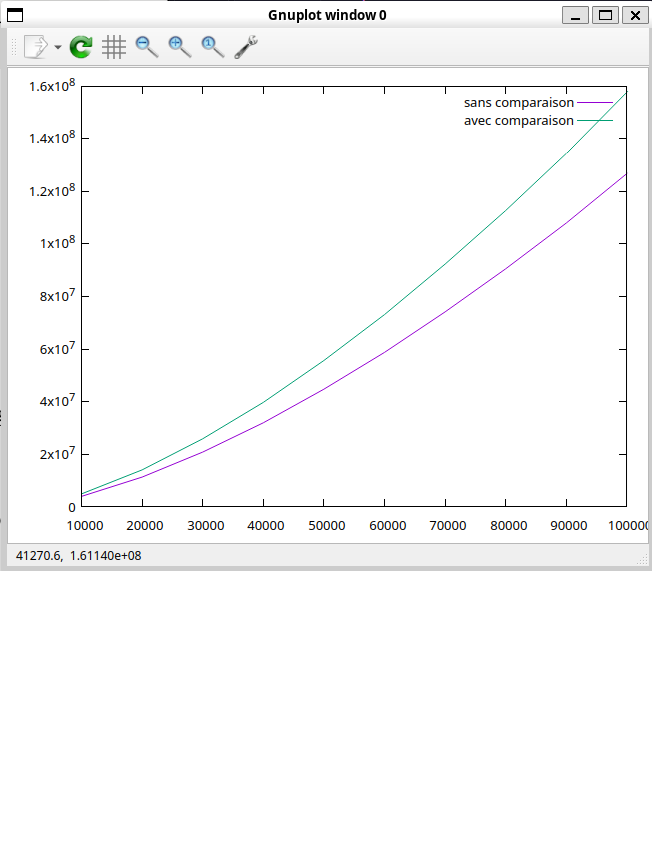
\includegraphics[width=8cm]{image_gnuplot_exo7.png}
\end{minipage}

\section*{\textbf{Exercice 8 : Bonus}}

\begin{lstlisting}[language=C, caption={Exo tri bulle et comparaisons recherche dichotomique}]
    #include <stdio.h>
#include <stdlib.h>
#include <assert.h>
#include <string.h>
#include <stdbool.h>

////// Exercice 8 : Bonus ///////


// Q1
void tri_bulle(int* tab, int n){
    int i = 0; 
    while(i<n){
        int j = i+1;
        while(j<n){
            if(tab[i]>tab[j]){
                int buff = tab[i]; 
                tab[i] = tab[j]; 
                tab[j] = buff; 
            } 
            j+=1; 
        }
        i+=1; 
    }
}

void affiche_tab(int* tab, int n){
    int i = 0; 
    while(i<n){
        printf("%d ", tab[i]);
        i+=1; 
    }
    printf("\n"); 
}

// Test Q1 

int main(int argc, char* argv[]){
    int n = 5; 
    
    int tab[5] = {1, 4, 2, 3, 0}; 

    tri_bulle(tab, n);
    
    affiche_tab(tab, n); 

    return 0;
}

// Q2 

// Conjecture : let's suppose we don't need the result anymore (0 or 1) but we only put our focus on nb_op
int is_elt(int* tab, int n, int x){
    int nb_op=0;

    int i = 0; 

    nb_op+=1; 

    while(i<n){
        if (x == tab[i]){
            return nb_op; 
        }
        i++; 
        nb_op+=4; 
    }
    return nb_op; 
}
// Same Conjecture here 
int is_elem_dich(int* tab, int n, int x){
    int nb_op = 0; 
    
    int debut = 0; 
    int fin = n-1; 

    nb_op+=2; 

    while(debut<fin){
        int mid = (debut+fin)/2; 
        if(tab[mid]==x){
            nb_op+=1;
            return nb_op;
        }
        if(x < tab[mid]){
            fin = mid-1; 
            nb_op+=2; 
        }
        else{
            debut = mid+1; 
            nb_op +=1; 
        }
        nb_op+=2; 
    }
    return nb_op; 
}

int main(int argc, char* argv[]){
    
    int n_min = 1000; 
    int n_max = 20000; 
    int pas   = 1000; 

    int n; 
    for(n = n_min; n <= n_max; n += pas){

        int* tab1 = malloc(n*sizeof(int)); 
        int indice1 = 0;
        while(indice1<n){
            tab1[indice1] = rand(); 
            indice1+=1; 
        }

        int x1 = rand();

        int nb_op_iter = is_elt(tab1, n, x1); 

        tri_bulle(tab1, n); 
        int nb_op_dich = is_elem_dich(tab1, n, x1);

        free(tab1); 

        printf("%d\t%d\t%d\n", n, nb_op_iter, nb_op_dich);
    }

    return 0;  
}
\end{lstlisting}

\subsection*{\textbf{GNUPLOT Test Exercice 8 :} \textit{Echelle y en log}}

\begin{minipage}[c]{10cm}
    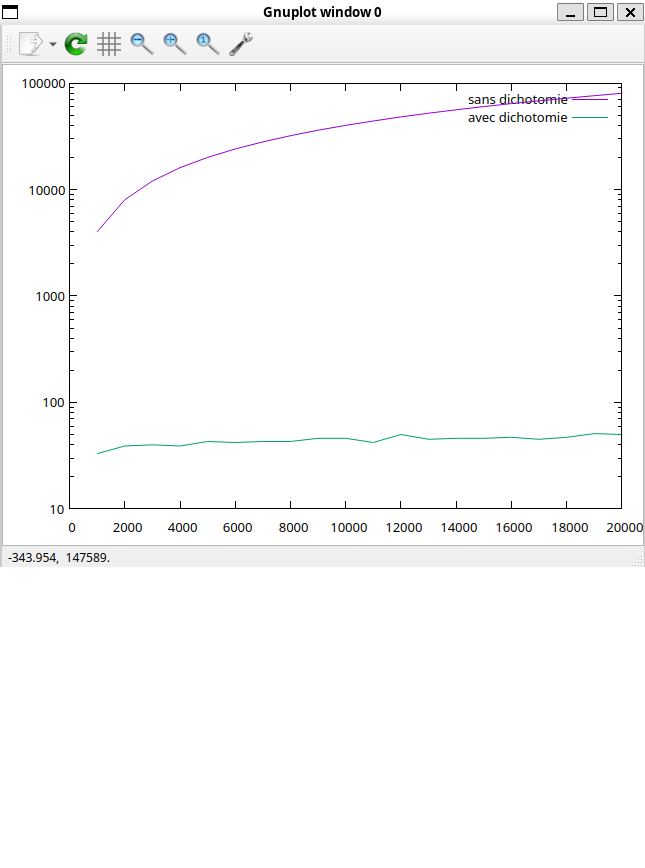
\includegraphics[width=8cm]{image_gnuplot_exo8_y_en_log.png}
\end{minipage}


\end{document}